\section{Resultados e discuss\~ao}\label{sec:resultados}

% Exemplo 1 (benchmark) JA EXECUTADO: texto e numeros preservados do
% grupo. Exemplos 2 e 3 com estrutura completa e placeholders \falta
% (a executar). Ver plano de melhorias para a defini\c{c}\~ao dos
% exemplos finais (RUL, manuten\c{c}\~ao, otimiza\c{c}\~ao, p_f vs limiar).

Os exemplos a seguir formam uma escada de evidência: o Exemplo~1 verifica o arcabouço metodológico em um problema de referência de baixo custo, no qual a solução de Monte Carlo direta serve de \textit{ground truth}; o Exemplo~2 aplica o emulador ao problema-alvo --- a previsão da RUL probabilística de uma viga de concreto armado sob corrosão induzida por carbonatação; e o Exemplo~3 estende a análise a um cenário com intervenção de manutenção, demonstrando o uso do emulador no suporte à decisão.

% =====================================================================
\subsection{Exemplo 1 --- Verifica\c{c}\~ao em problema de refer\^encia}
\label{subsec:exemplo1}
% =====================================================================

Para verificar o arcabouço metodológico proposto, adota-se uma versão adaptada do problema de referência introduzido por \textcite{pires2024}, definida pela Equação~\eqref{eq:toy_problem_equation}. Nessa formulação, $\mathbf{R}$ e $\mathbf{S}$ denotam, respectivamente, a resistência estrutural e a solicitação. A dependência temporal é introduzida por um fator de degradação linear aplicado à resistência, $k_{\mathrm{fator}}(t)$, que modela a redução progressiva da capacidade ao longo da vida útil, com $k_{\mathrm{inicial}} = 1{,}0$ no instante inicial e $k_{\mathrm{final}} = 0{,}3$ ao final do horizonte $T_f = 100$ anos, conforme a Equação~\eqref{eq:k_factor_linear}. As incertezas de modelagem são incorporadas pelas variáveis latentes $\mathbf{Z}_1$ e $\mathbf{Z}_2$, que afetam resistência e solicitação:

\begin{equation}
k_{\mathrm{fator}}(t) =
\begin{cases}
k_{\mathrm{inicial}}, & t \leq 0 \\[5pt]
k_{\mathrm{final}}, & t \geq T_f \\[5pt]
k_{\mathrm{inicial}} + (k_{\mathrm{final}} - k_{\mathrm{inicial}}) \cdot \dfrac{t}{T_f}, & 0 < t < T_f
\end{cases}
\label{eq:k_factor_linear}
\end{equation}

\begin{equation}
g(\mathbf{R}, \mathbf{S}, t) = k_{\mathrm{fator}}(t) \cdot \frac{\mathbf{R}}{\mathbf{Z}_1} - \mathbf{S} \cdot \mathbf{Z}_2
\label{eq:toy_problem_equation}
\end{equation}

\begin{table}[H]
\centering
\caption{Parâmetros estatísticos e distribuições de probabilidade das variáveis do problema de referência.}
\label{tab:random_variables_parameters}
\begin{tabular}{l c c c c}
\hline
\textbf{Variável} & \textbf{Símbolo} & \textbf{Distribuição} & \textbf{Média} & \textbf{Desvio padrão} \\
\hline
Resistência                          & $R$     & Normal     & 5,00 & 0,80  \\
Solicitação                          & $S$     & Normal     & 2,00 & 0,60  \\
Incerteza de modelo (resistência)    & $Z_1$   & Lognormal  & 1,00 & 0,028 \\
Incerteza de modelo (solicitação)    & $Z_2$   & Lognormal  & 1,00 & 0,096 \\
\hline
\end{tabular}
\end{table}

\subsubsection{Comportamento temporal dos par\^ametros da GLD}

A análise dependente do tempo considera 10 passos igualmente espaçados em um horizonte de 100 anos. Em cada passo, realizações da função de estado limite são avaliadas e os quatro parâmetros da GLD, $\lambda_1$ a $\lambda_4$, são ajustados via PyGLAM. Para fins ilustrativos, realizações fixas $r = 5{,}09$ e $s = 1{,}80$ são consideradas, com 2.000 amostras das variáveis latentes por passo de tempo. A Figura~\ref{fig:g_function_realizations} mostra a evolução temporal da função de estado limite, refletindo claramente a influência do fator de degradação, e a correspondente evolução dos parâmetros da GLD.

\begin{figure}[H]
    \centering
    \begin{subfigure}{0.9\textwidth}
        \centering
        
\includegraphics[width=\textwidth]{z_time-lapse_g_analysis_en.png}
        \caption{}
        \label{fig:g_realizacoes}
    \end{subfigure}
    \vspace{0.3cm}
    \begin{subfigure}{0.95\textwidth}
        \centering
        
\includegraphics[width=\textwidth]{z_lambdas_for_r_s_realization_en.png}
        \caption{}
        \label{fig:lambdas_tempo}
    \end{subfigure}
    \caption{Avaliação da função $g$ ao longo do tempo. (A) Realizações com valores fixos $r = 5{,}09$ e $s = 1{,}80$. (B) Evolução de $\lambda_1$--$\lambda_4$ no tempo. \falta{traduzir rótulos das figuras}}
    \label{fig:g_function_realizations}
\end{figure}

Previamente ao treinamento do metamodelo, conduziu-se uma avaliação exploratória da sensibilidade dos parâmetros da GLD: 1.000 realizações de $r$ e $s$, combinadas a 2.000 amostras das variáveis latentes, foram analisadas em $t = 0$ e $t = 50$ anos. Os resultados demonstram que $\lambda_1$ e $\lambda_2$ apresentam sensibilidade pronunciada às variações de $\mathbf{R}$ e $\mathbf{S}$, enquanto $\lambda_3$ e $\lambda_4$ exibem baixa dispersão e fraca dependência das entradas. Com base nessa evidência, apenas $\lambda_1$ e $\lambda_2$ foram selecionados como variáveis-alvo do treinamento, sendo $\lambda_3$ e $\lambda_4$ representados por seus valores médios. A Tabela~\ref{tab:validation_results} confirma a decisão: os altos valores de $R^2$ obtidos para $\lambda_1$ e $\lambda_2$ em todos os passos de tempo indicam excelente acurácia preditiva da PCE, enquanto os valores consistentemente baixos para $\lambda_3$ e $\lambda_4$ corroboram sua exclusão do treinamento.

\begin{table}[H]
\centering
\caption{Validação estatística do metamodelo PCE em diferentes passos de tempo (valores de $R^2$).}
\label{tab:validation_results}
\begin{tabular}{rrrrr}
\toprule
Tempo (anos) & $\lambda_1$ & $\lambda_2$ & $\lambda_3$ & $\lambda_4$ \\
\midrule
0   & 1,0000 & 0,9839 & 0,3858 & 0,3978 \\
20  & 1,0000 & 0,9894 & 0,3713 & 0,3804 \\
40  & 1,0000 & 0,9792 & 0,4081 & 0,3891 \\
60  & 1,0000 & 0,9926 & 0,3102 & 0,3525 \\
80  & 1,0000 & 0,9918 & 0,2277 & 0,2146 \\
100 & 1,0000 & 0,9865 & 0,0638 & 0,1352 \\
\bottomrule
\multicolumn{5}{l}{\footnotesize \textit{Nota: tabela condensada; a versão completa com os 11 passos consta de \falta{apêndice/material suplementar}.}}
\end{tabular}
\end{table}

\subsubsection{Qualidade da distribui\c{c}\~ao emulada}

A Figura~\ref{fig:kde_comparison} compara, por estimativa de densidade por núcleo (KDE), a distribuição de referência (\textit{ground truth}) e a aproximação GLaM obtida via PCE para as realizações fixas $r = 5{,}09$ e $s = 1{,}80$, em $t = 0$ e $t = 50$ anos.

\begin{figure}[H]
    \centering
    \begin{subfigure}[b]{0.38\textwidth}
        \centering
        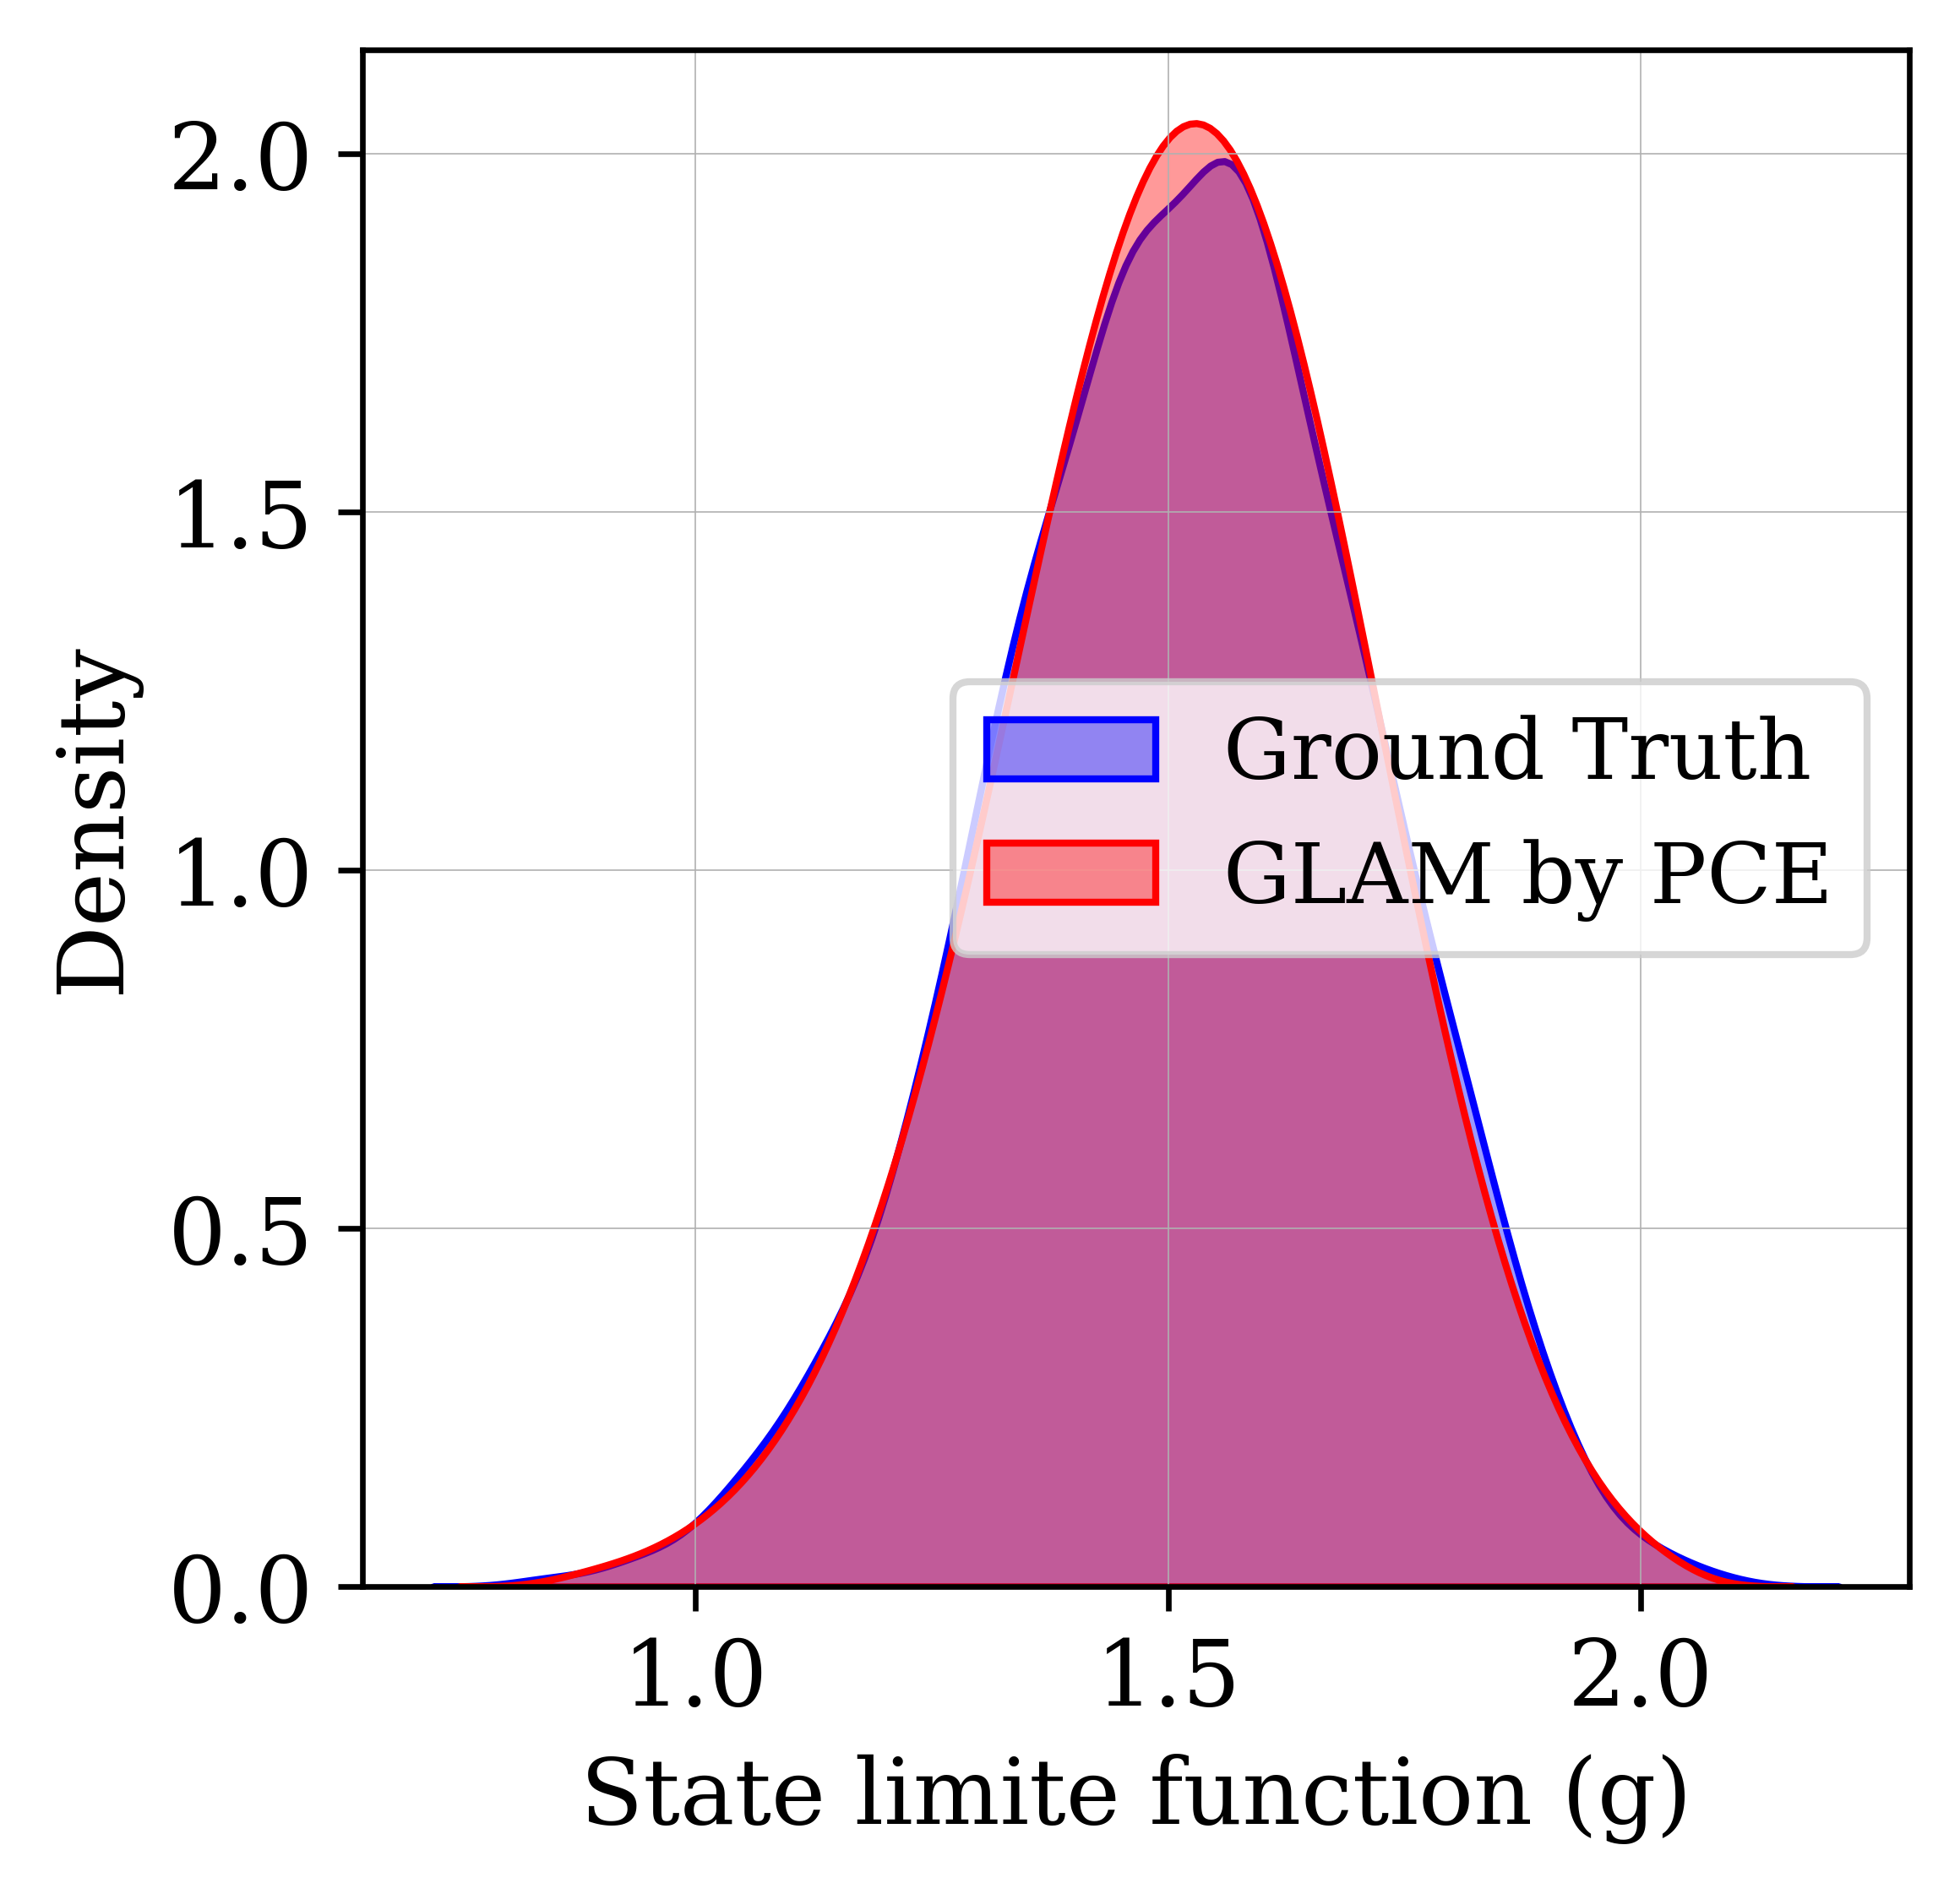
\includegraphics[width=\textwidth]{z_histogram_glam_versus_gt_t0_en.png}
        \caption{$t=0$}
        \label{fig:kde_t0}
    \end{subfigure}
    \hfill
    \begin{subfigure}[b]{0.38\textwidth}
        \centering
        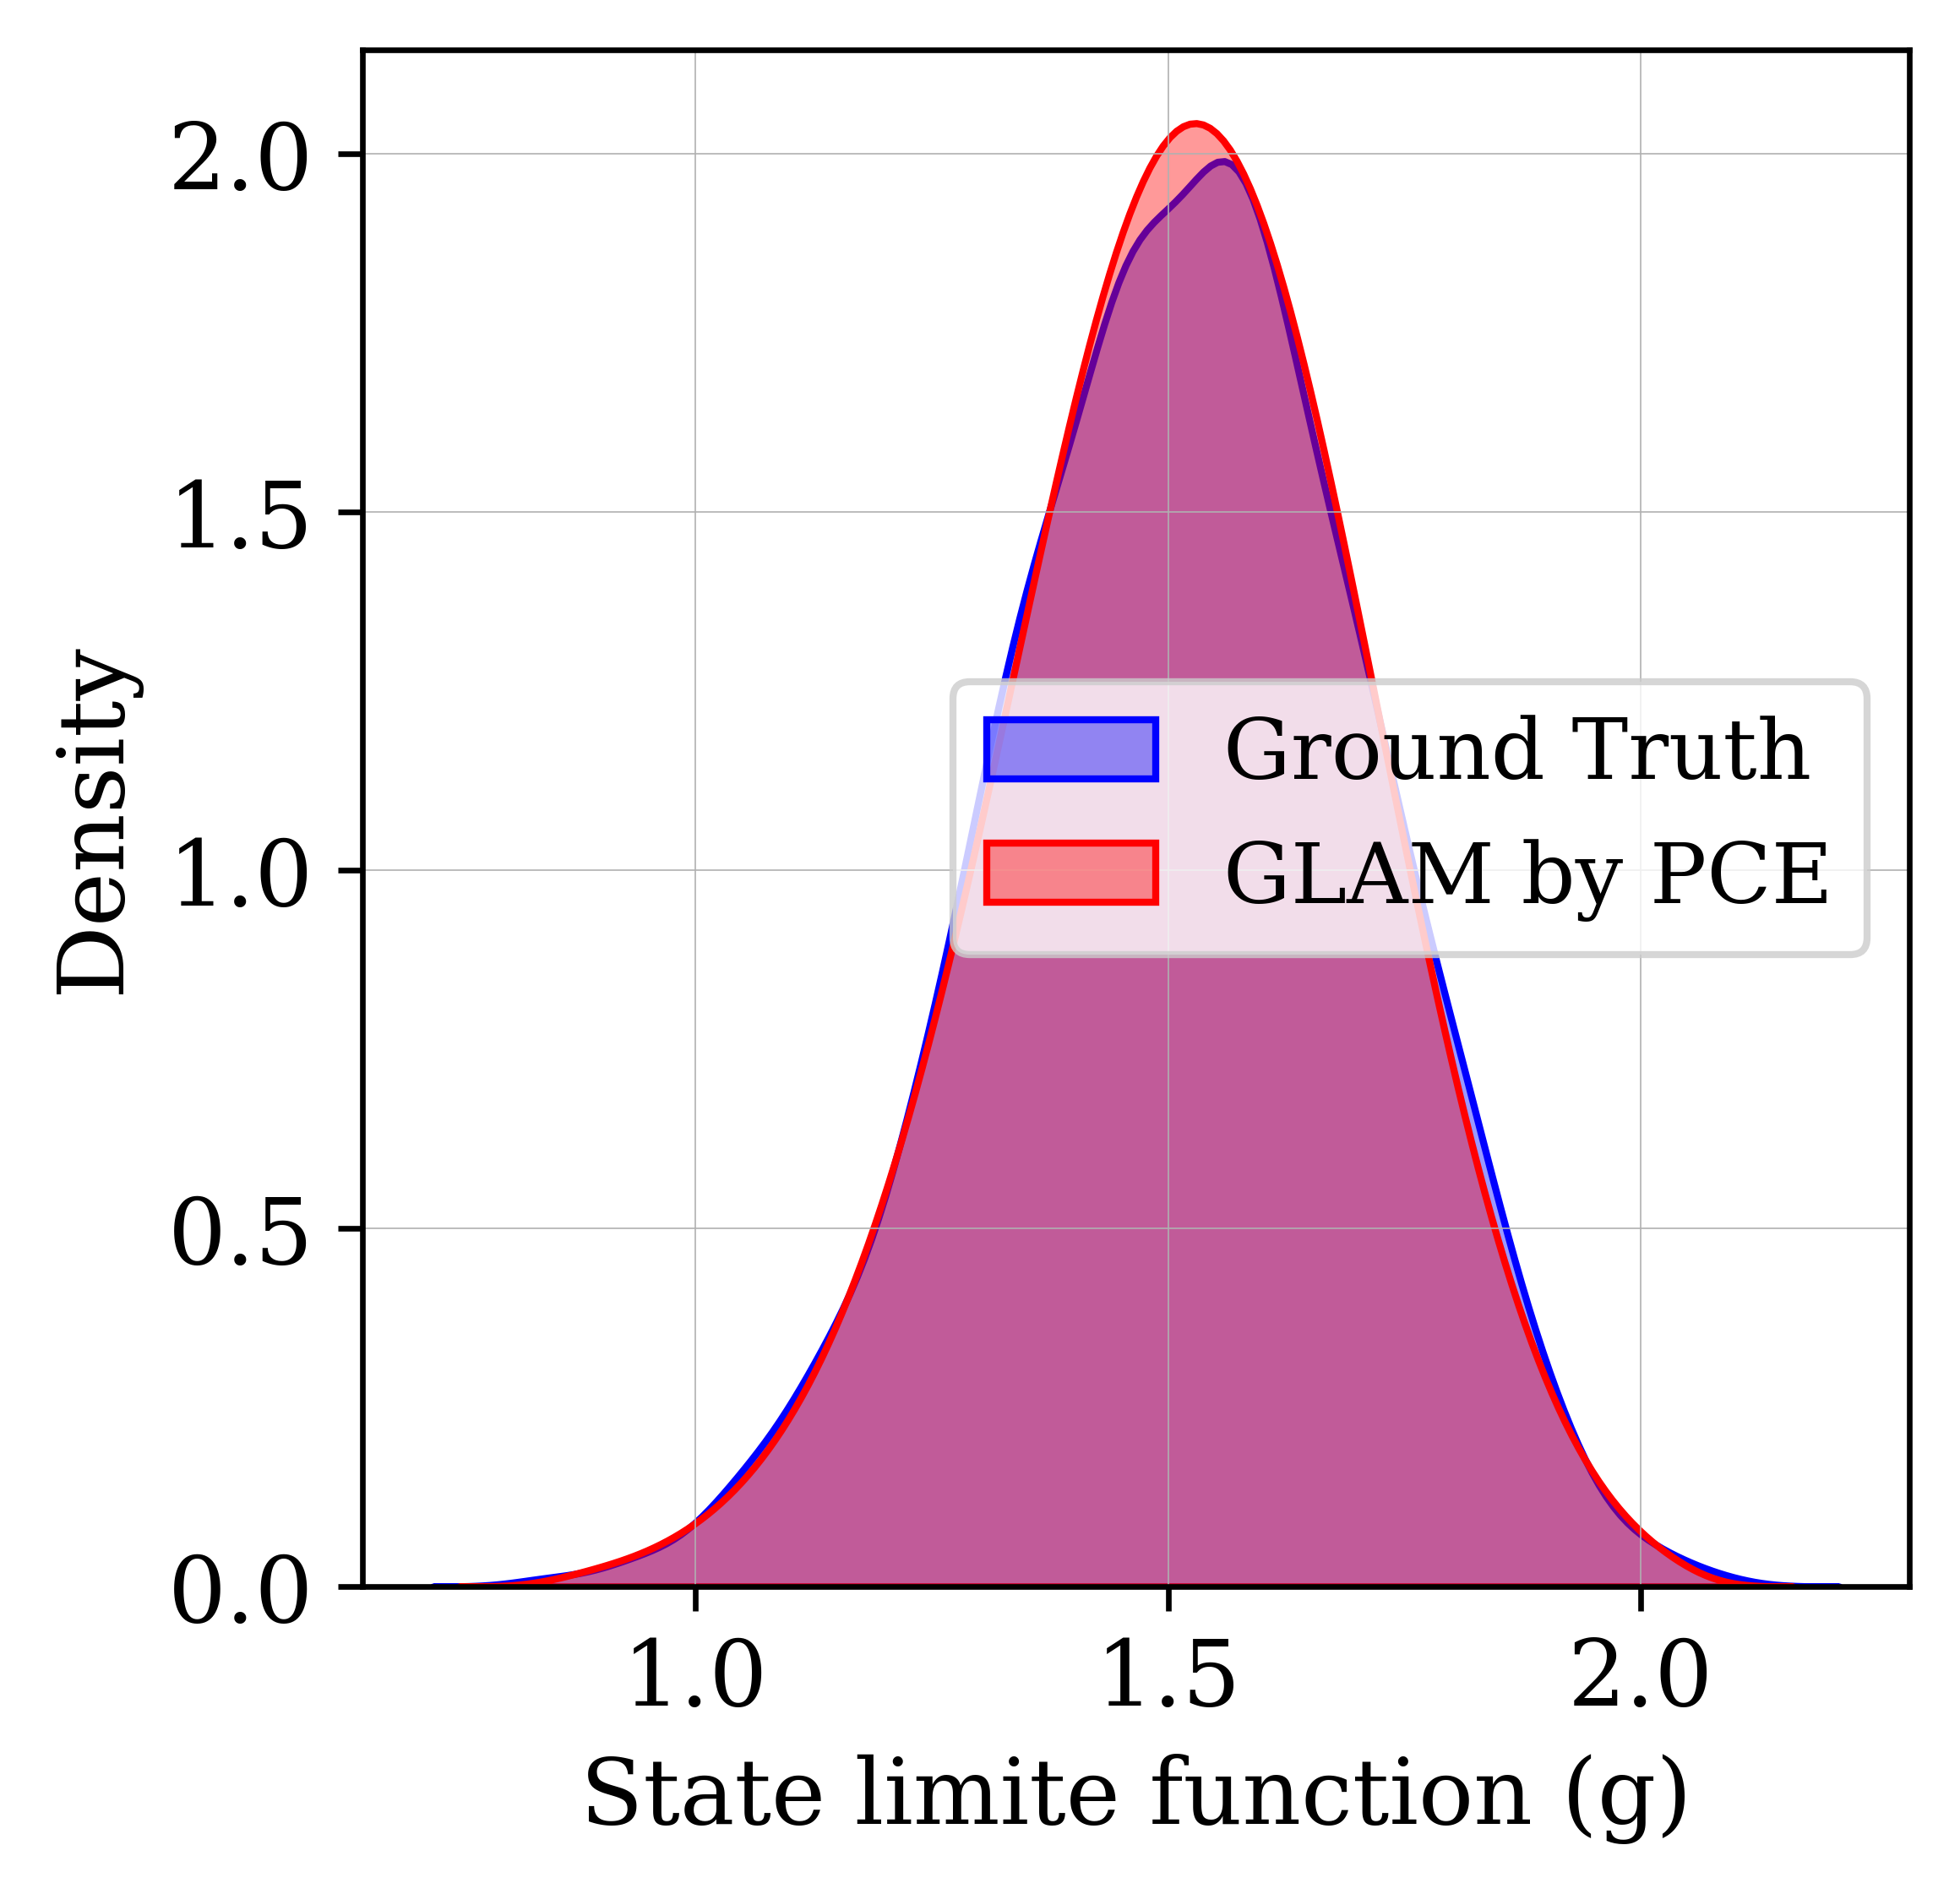
\includegraphics[width=\textwidth]{z_histogram_glam_versus_gt_t50_en.png}
        \caption{$t=50$ anos}
        \label{fig:kde_t50}
    \end{subfigure}
    \caption{Comparação entre a referência (\textit{ground truth}) e a aproximação GLaM via KDE, para as realizações fixas $r=5{,}09$ e $s=1{,}80$. \falta{traduzir rótulos das figuras}}
    \label{fig:kde_comparison}
\end{figure}

A similaridade estatística foi quantificada pelos testes de aderência e pela comparação de quantis descritos na Seção~\ref{subsec:metricas}, com resultados nas Tabelas~\ref{tab:statistical_tests} e \ref{tab:quantile_comparison}. O teste KS não rejeita a hipótese nula ao nível de 5\% ($D = 0{,}0108$; valor-p $= 0{,}9325$), indicando excelente concordância global entre as funções de distribuição empíricas. O teste AD, em contraste, rejeita a hipótese nula, comportamento atribuído à sua elevada sensibilidade às caudas em amostras grandes \parencite{scholz1987}. A análise de quantis localiza a origem da discrepância: os erros relativos permanecem abaixo de 0,5\% até o percentil 99, subindo a cerca de 1,3\% apenas no quantil extremo de 99,9\% --- desvio confinado à cauda e usualmente considerado aceitável em análises de confiabilidade e quantificação de incertezas \parencite{sudret2008}.

\begin{table}[H]
\centering
\caption{Resultados dos testes de Kolmogorov--Smirnov e Anderson--Darling para a comparação entre a referência (GT) e o emulador (GLaM).}
\label{tab:statistical_tests}
\begin{tabular}{lcccc}
\hline
Teste & Estatística & valor-p & Nível ($\alpha$) & Decisão \\
\hline
Kolmogorov--Smirnov & 0,0108 & 0,9325 & 0,05 & Não rejeita $H_0$ \\
Anderson--Darling   & $-0{,}6492$ & 0,0025 & 0,05 & Rejeita $H_0$ \\
\hline
\end{tabular}
\end{table}

\begin{table}[H]
\centering
\caption{Comparação de quantis entre a referência (GT) e o emulador (GLaM).}
\label{tab:quantile_comparison}
\begin{tabular}{ccccc}
\hline
Quantil & GT & GLaM & Diferença absoluta & Diferença relativa (\%) \\
\hline
0,001 & 0,8995 & 0,9037 & 0,0042 & 0,47 \\
0,010 & 1,0387 & 1,0393 & 0,0006 & 0,06 \\
0,500 & 1,5222 & 1,5198 & 0,0024 & 0,16 \\
0,990 & 1,9374 & 1,9356 & 0,0018 & 0,09 \\
0,999 & 2,0529 & 2,0263 & 0,0266 & 1,30 \\
\hline
\end{tabular}
\end{table}

\falta{adicionar à análise a divergência de Kullback--Leibler (Eq.~\ref{eq:kl_continua}) e/ou a distância de Wasserstein entre GT e GLaM, para alinhamento com a Seção~\ref{subsec:metricas}}

\subsubsection{Camada temporal de aprendizado de m\'aquina}

Partindo da análise em passos discretos via PCE, uma rede neural artificial (RNA) foi adotada para viabilizar a predição contínua dos parâmetros $\lambda_1$ e $\lambda_2$ ao longo da vida útil. Para o treinamento, uma base sintética de 11.000 amostras foi gerada com os metamodelos PCE previamente validados, amostrando-se o espaço de entrada segundo as distribuições da Tabela~\ref{tab:random_variables_parameters} e valores de tempo uniformemente distribuídos no horizonte de análise. A rede mapeia o vetor de entrada $\mathbf{x} = \{R, S, t\}$ no vetor de saída $\mathbf{y} = \{\lambda_1, \lambda_2\}$, com partição aleatória em subconjuntos de treinamento e teste.

A Figura~\ref{fig:ann_temporal} ilustra a evolução temporal de $\lambda_1$ e $\lambda_2$ ao longo dos 100 anos de vida útil, prevista pela RNA treinada para o cenário representativo ($r=5{,}09$, $s=1{,}80$). A rede atua como interpolador contínuo, reconstruindo suavemente a trajetória de degradação entre os passos discretos originalmente avaliados pela PCE, sem ruído numérico ou descontinuidades. Quantitativamente, o modelo atingiu $R^2 = 0{,}9976$ para $\lambda_1$ e $R^2 = 0{,}9844$ para $\lambda_2$ no conjunto de teste, validando a RNA como interpolador robusto para a avaliação contínua da confiabilidade em qualquer instante do horizonte. \falta{acrescentar o teste crítico de generalização temporal: treinar a RNA OMITINDO um ou dois passos de tempo (ex.: 35 e 65 anos) e comparar a PDF prevista nesses anos com Monte Carlo direto --- este é o experimento que sustenta a alegação de emulação temporal; reportar KS/quantis para os anos omitidos}

\begin{figure}[H]
    \centering
    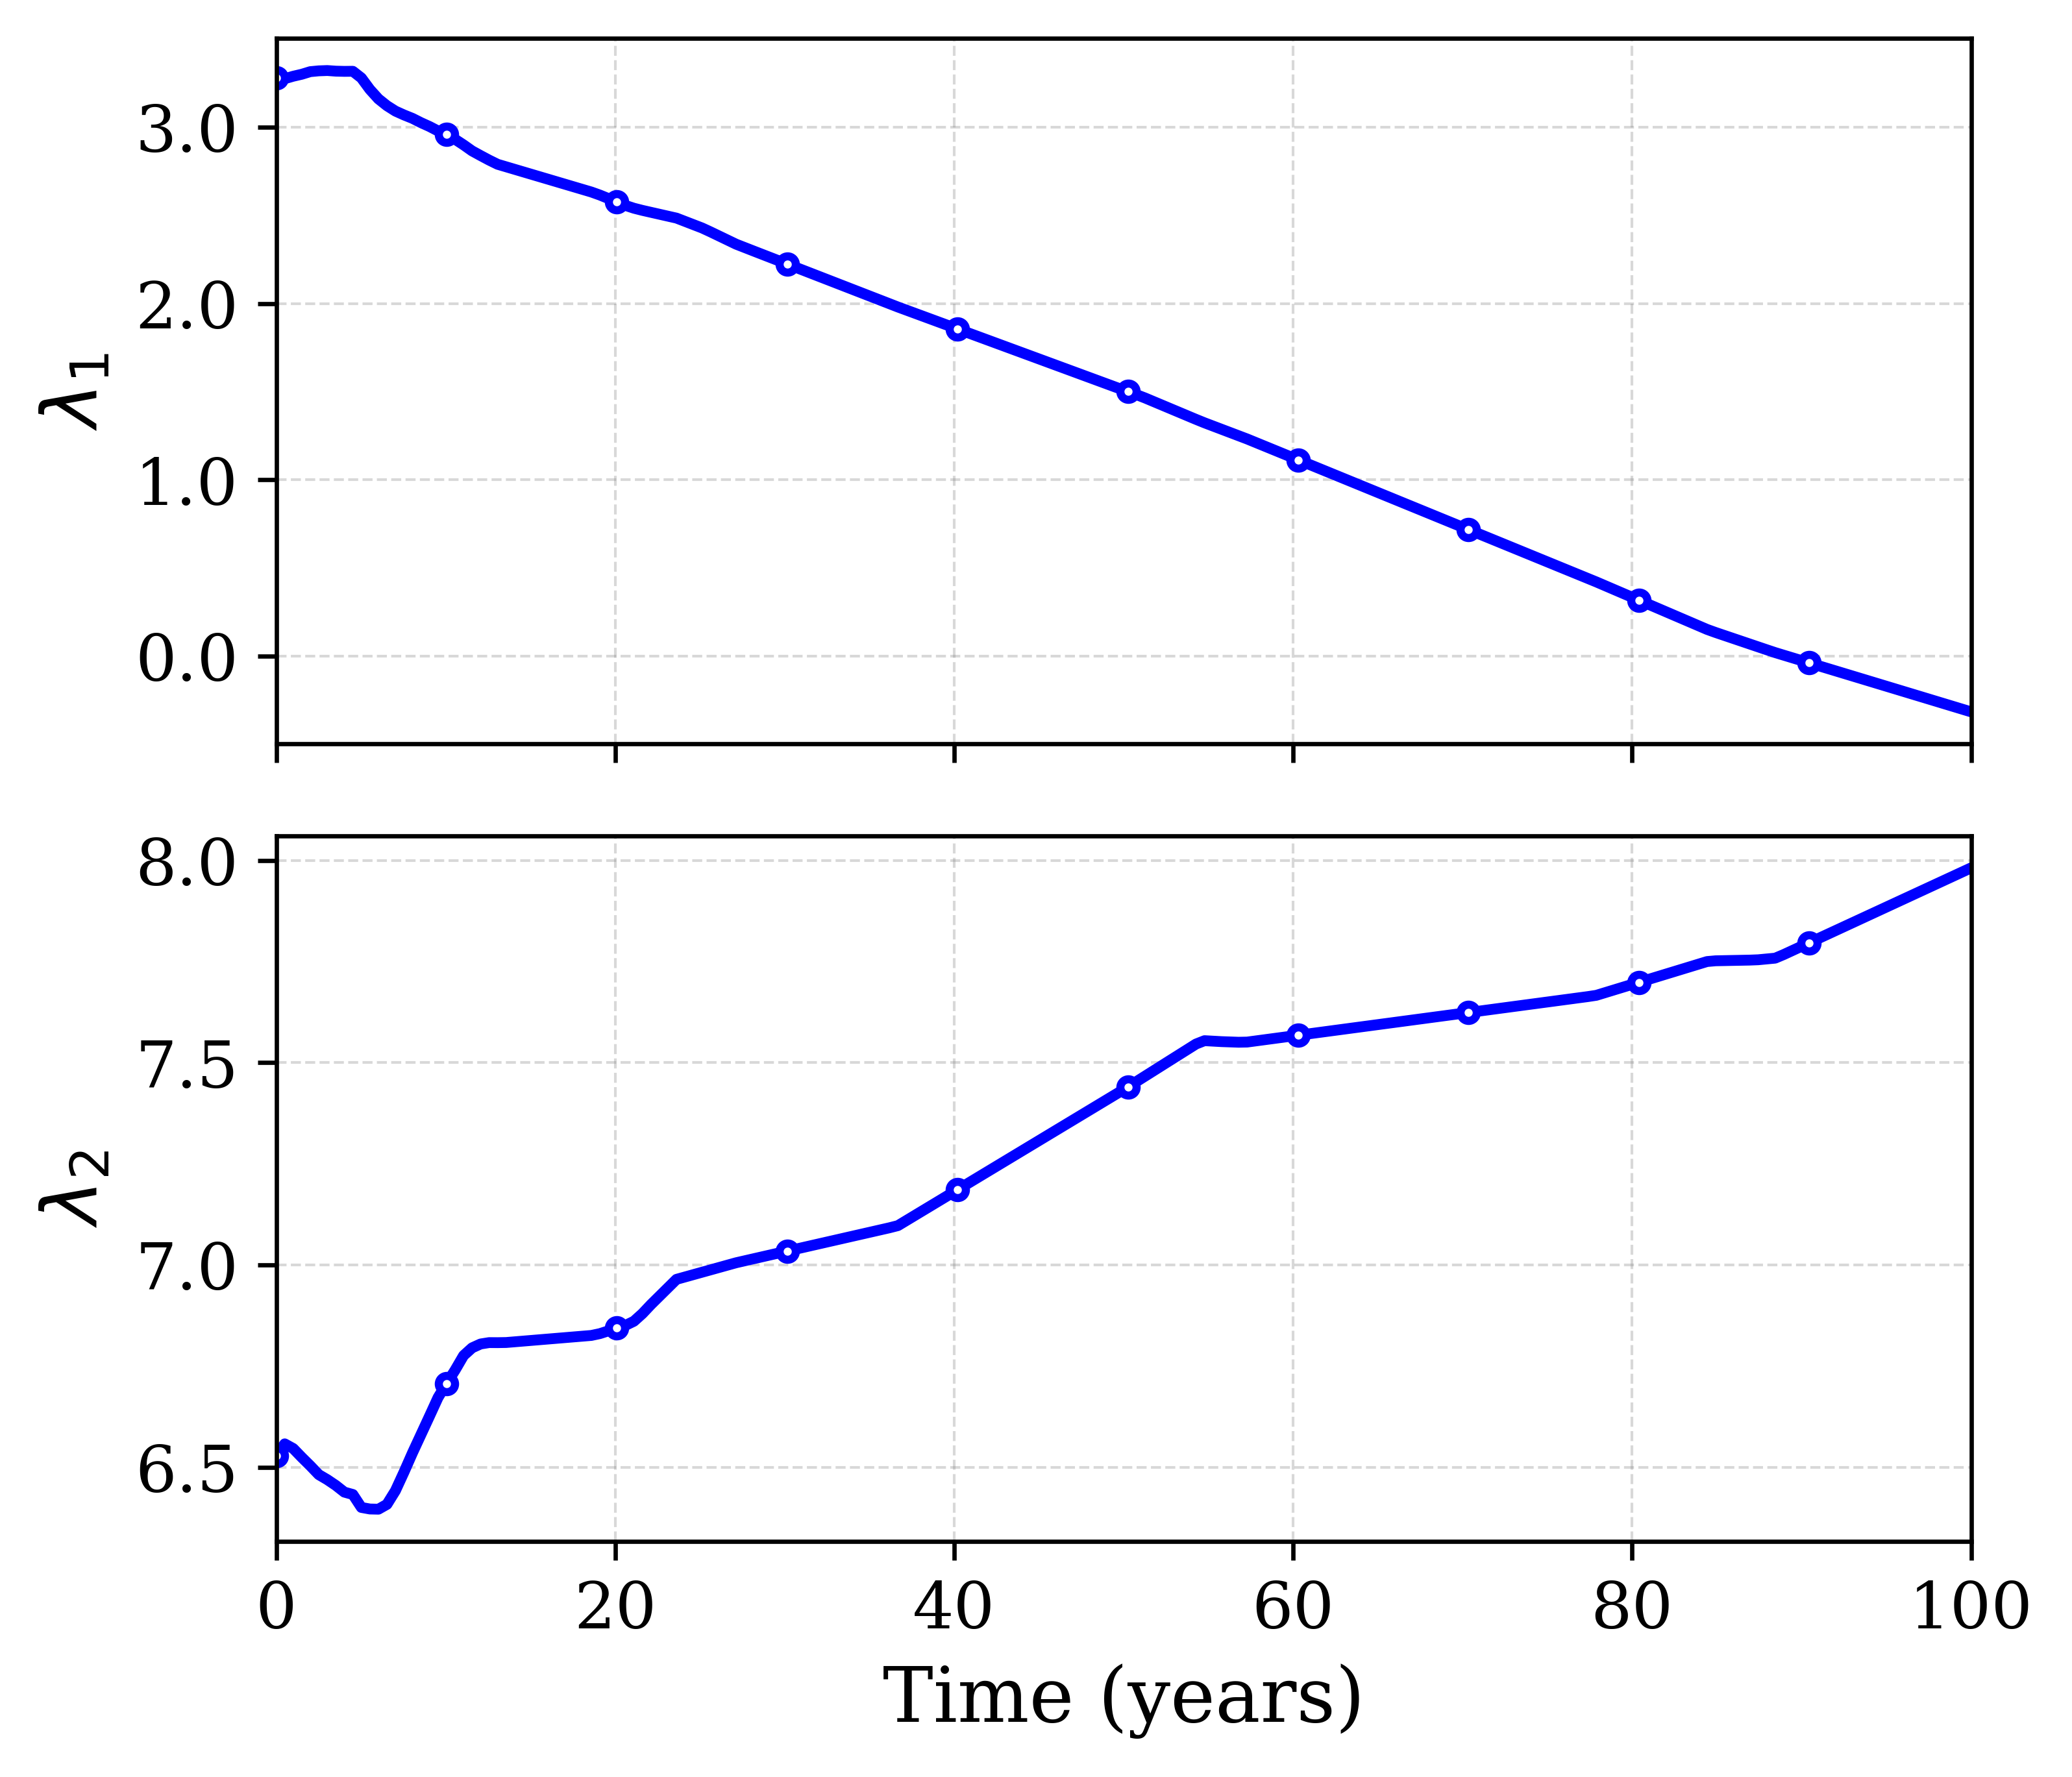
\includegraphics[width=0.75\linewidth]{z_temporal_evolution_ann_with_points_en.png}
    \caption{Evolução temporal dos parâmetros $\lambda_1$ e $\lambda_2$ ao longo da vida útil ($t \in [0, 100]$ anos) para a realização fixa $r = 5{,}09$ e $s = 1{,}80$. As linhas contínuas representam a interpolação por RNA. \falta{traduzir rótulos da figura}}
    \label{fig:ann_temporal}
\end{figure}

\subsubsection{Vida \'util remanescente e custo computacional}

Aplicando a metodologia da Seção~\ref{subsec:rul}, a Figura~\ref{fig:rul_results} apresenta os produtos probabilísticos do arcabouço: (a) a distribuição da função de estado limite no instante de inspeção de 35 anos, adotado como exemplo representativo; (b) a densidade de probabilidade do tempo até a falha, obtida pela identificação do instante em que a trajetória de $g$ se anula (Eq.~\ref{eq:ttf}); e (c) a distribuição resultante da RUL (Eq.~\ref{eq:rul}), que consolida as incertezas propagadas e constitui o resultado-chave para manutenção preditiva.

\begin{figure}[H]
    \centering
    \begin{subfigure}[b]{0.32\textwidth}
        \centering
        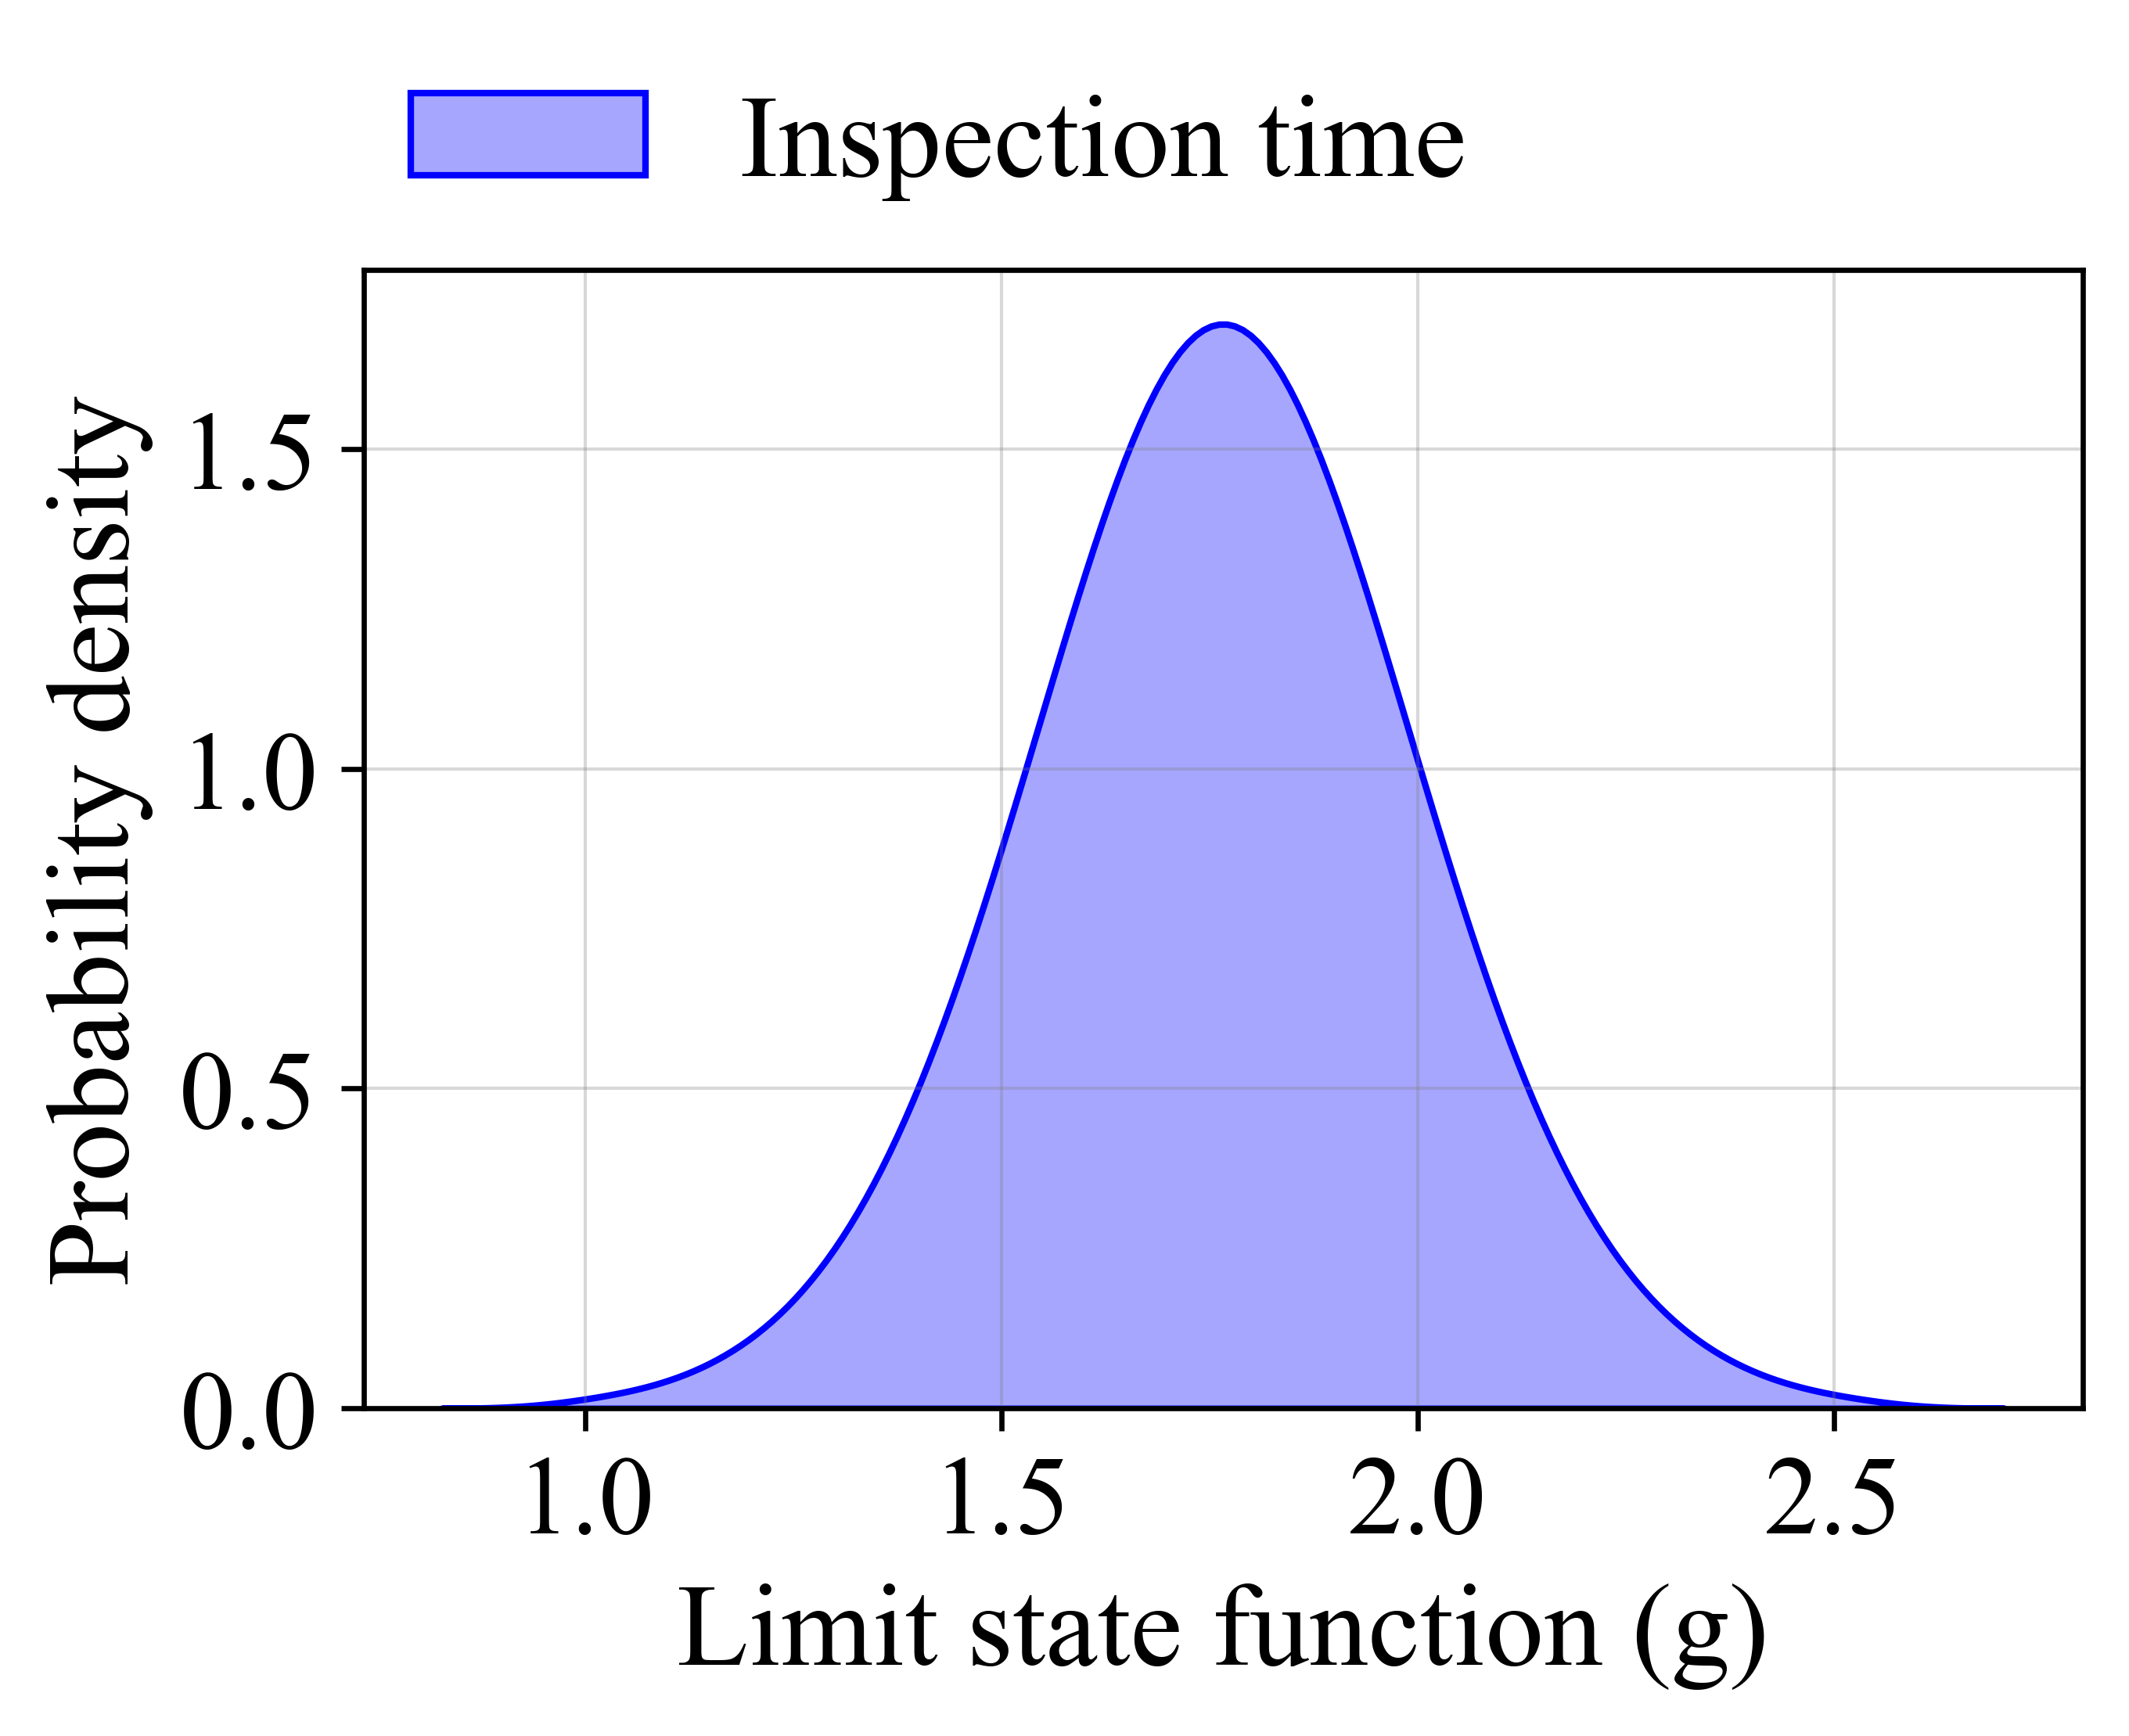
\includegraphics[height=4.0cm,keepaspectratio]{z_kde_inspection_time.png}
        \caption{KDE de $g$ no instante de inspeção.}
        \label{fig:kde_inspection_time}
    \end{subfigure}
    \hfill
    \begin{subfigure}[b]{0.32\textwidth}
        \centering
        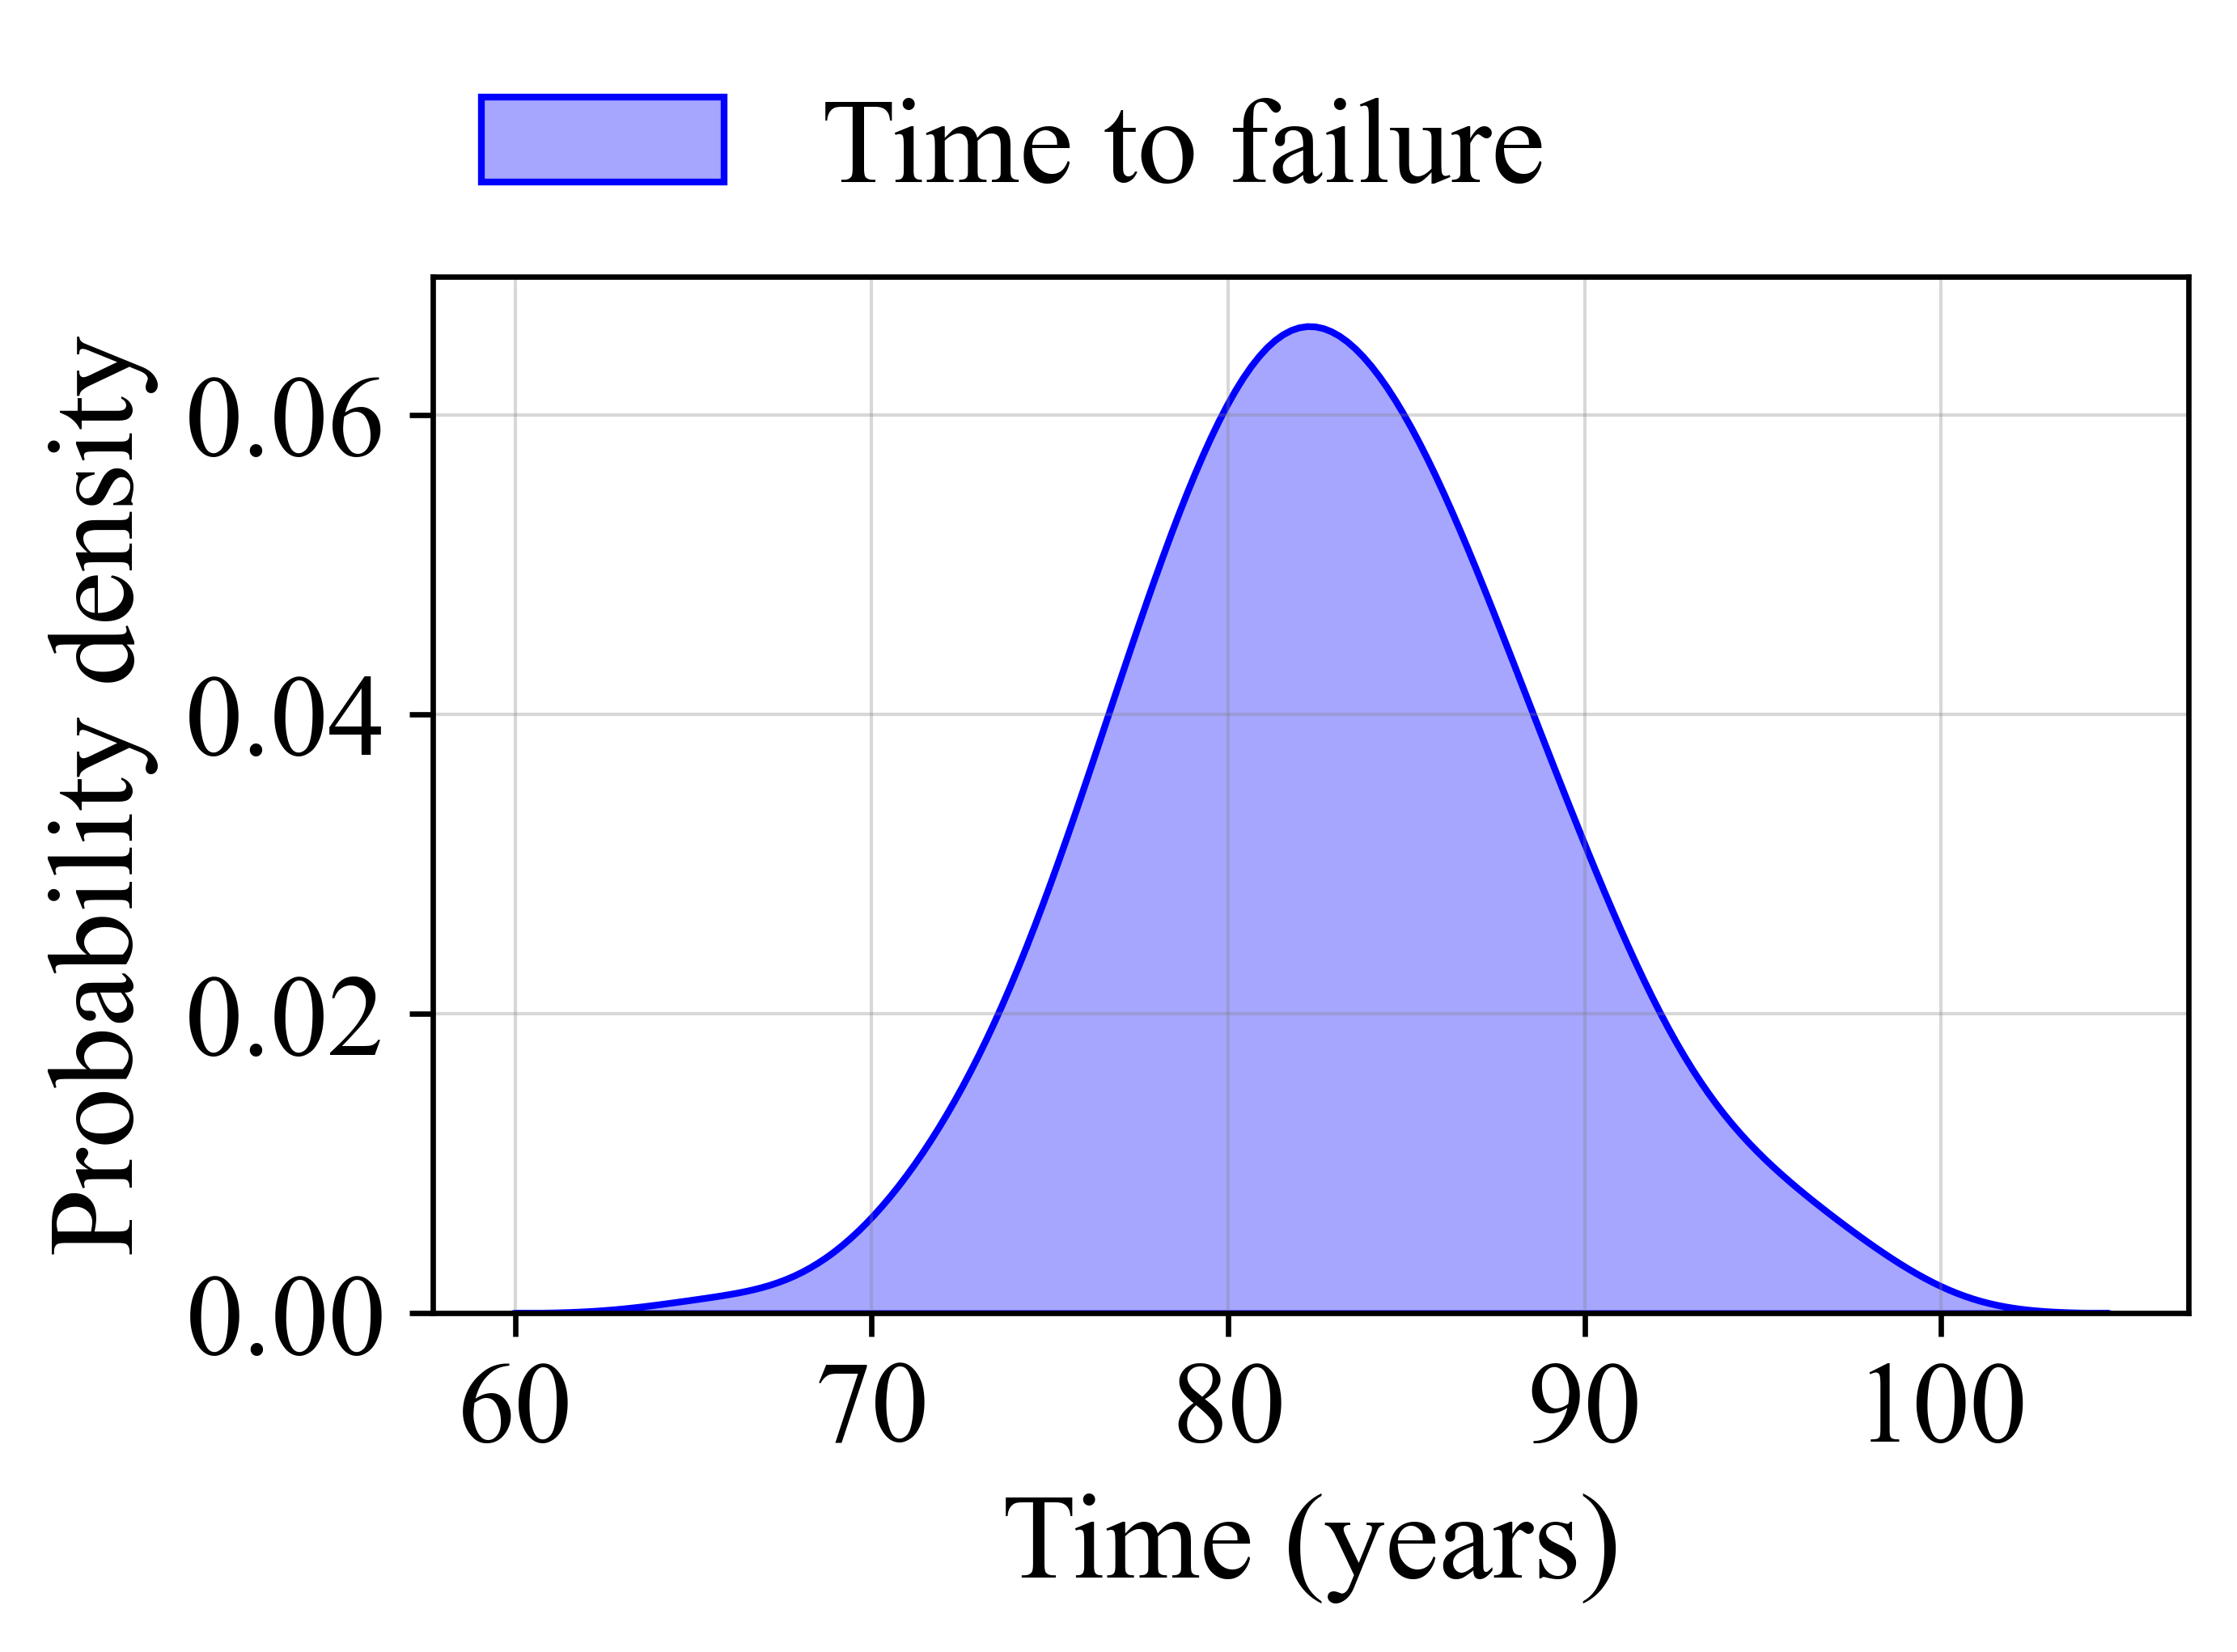
\includegraphics[height=4.0cm,keepaspectratio]{z_kde_time_to_failure.png}
        \caption{Densidade do tempo até a falha.}
        \label{fig:kde_time_to_failure}
    \end{subfigure}
    \hfill
    \begin{subfigure}[b]{0.32\textwidth}
        \centering
        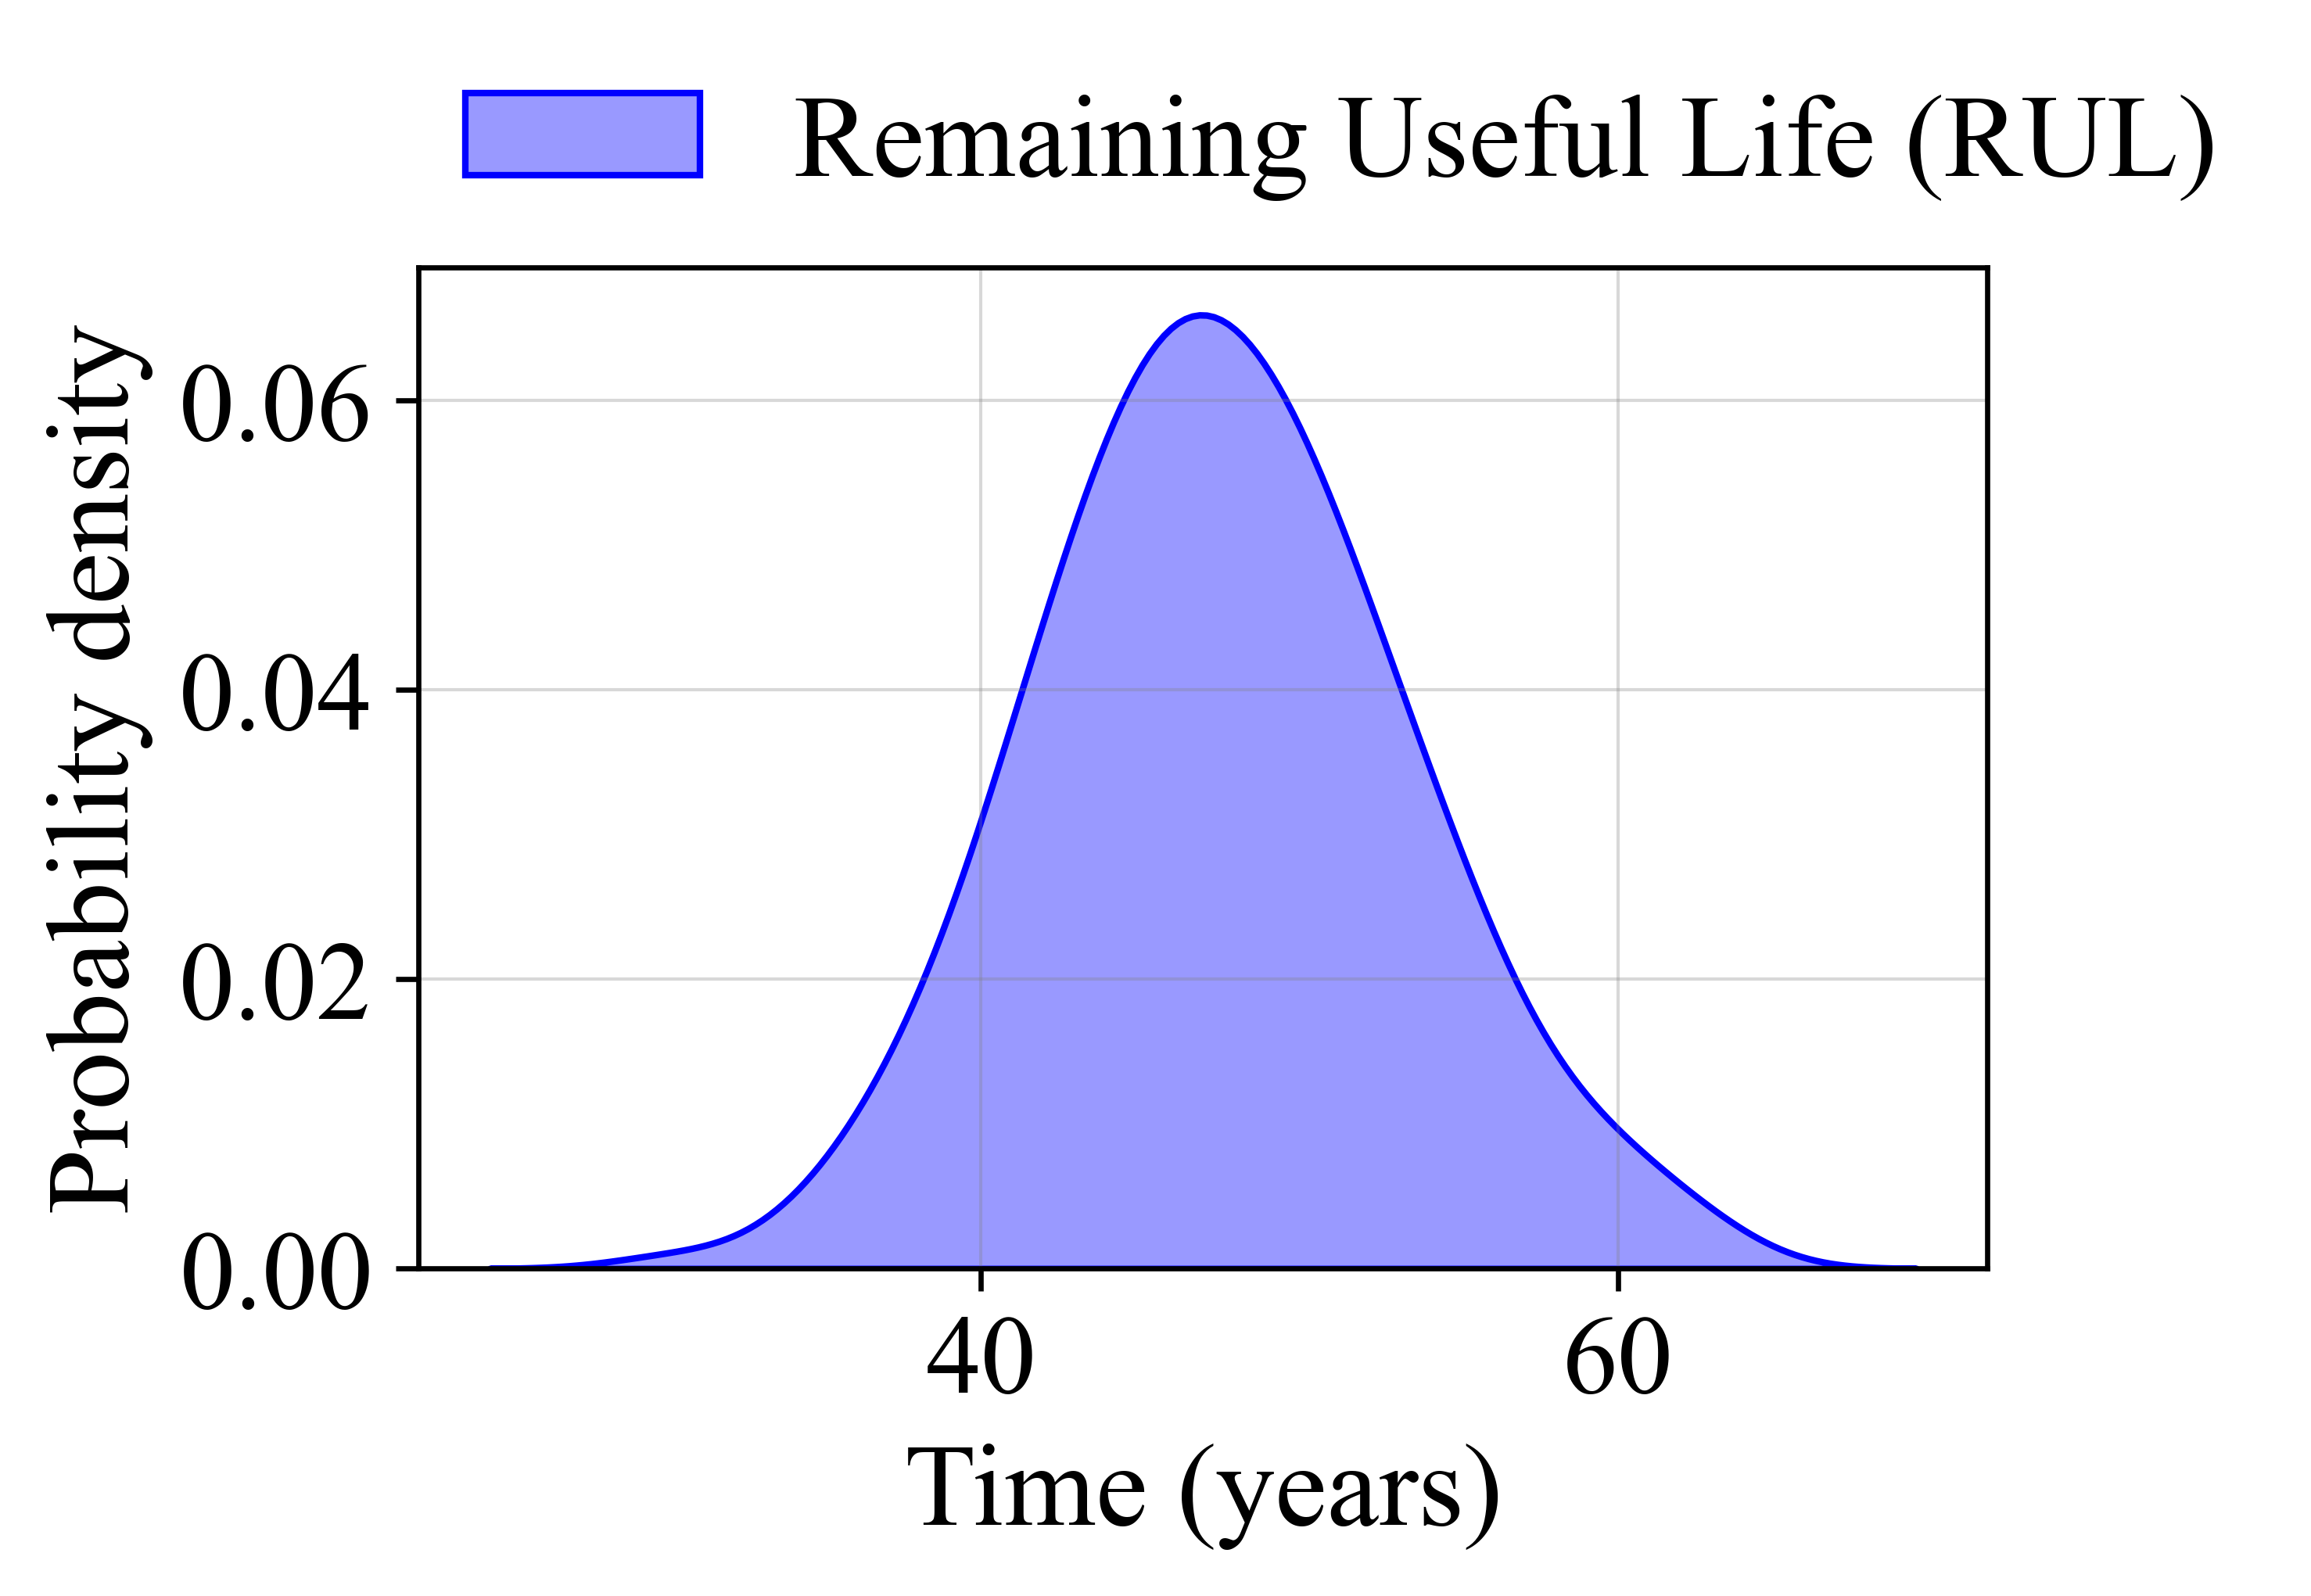
\includegraphics[height=4.0cm,keepaspectratio]{z_kde_rul.png}
        \caption{KDE da vida útil remanescente.}
        \label{fig:kde_rul}
    \end{subfigure}
    \caption{Resultados probabilísticos do arcabouço baseado em emulador para a estimativa de RUL: (A) distribuição da função de estado limite no instante de inspeção ($t_{\mathrm{insp}} = 35$ anos), (B) distribuição do tempo até a falha e (C) distribuição resultante da RUL. \falta{traduzir rótulos das figuras}}
    \label{fig:rul_results}
\end{figure}

As métricas de risco derivadas da distribuição de RUL para $\alpha = 5\%$ são apresentadas na Tabela~\ref{tab:var_cvar_rul}. A diferença relativamente pequena entre VaR e CVaR sugere severidade de cauda limitada, indicando que, mesmo em condições desfavoráveis, a vida remanescente prevista não exibe degradação abrupta.

\begin{table}[H]
\centering
\caption{Métricas de risco derivadas da distribuição de RUL para $\alpha = 5\%$ (Exemplo 1).}
\label{tab:var_cvar_rul}
\begin{tabular}{lc}
\hline
\textbf{Métrica} & \textbf{Valor (anos)} \\
\hline
VaR$_{5\%}$  & 38,38 \\
CVaR$_{5\%}$ & 36,42 \\
\hline
\end{tabular}
\end{table}

Além da acurácia das predições probabilísticas, o arcabouço oferece ganho substancial de eficiência computacional. A Tabela~\ref{tab:computational_time} compara o tempo de processamento exigido pela abordagem convencional e pelo emulador: enquanto o procedimento convencional demandou aproximadamente 48,75~s, o emulador reduziu o custo a apenas 0,66~s, correspondendo a um \textit{speed-up} de quase duas ordens de grandeza. Esse resultado evidencia a adequação da abordagem a análises de confiabilidade e RUL em tempo quase real ou em larga escala.

\begin{table}[H]
\centering
\caption{Comparação do tempo computacional entre a abordagem convencional e a baseada em emulador (Exemplo 1).}
\label{tab:computational_time}
\begin{tabular}{l c}
\hline
\textbf{Método} & \textbf{Tempo computacional (s)} \\
\hline
Abordagem convencional & 48,75 \\
Abordagem com emulador & 0,66 \\
\hline
\end{tabular}
\end{table}

% =====================================================================
\subsection{Exemplo 2 --- RUL probabil\'istica de viga de concreto armado sob carbonata\c{c}\~ao}
\label{subsec:exemplo2}
% =====================================================================

Verificado o arcabouço, aplica-se o emulador ao problema-alvo: a previsão da vida útil remanescente de uma viga de concreto armado sujeita à corrosão induzida por carbonatação, com a função de estado limite da Equação~\eqref{eq:funcao_g} e os modelos físicos das Seções~\ref{subsec:carbonatacao} e \ref{subsec:resistencia_residual}.

\subsubsection{Defini\c{c}\~ao do problema}

A viga analisada possui seção retangular com os parâmetros geométricos e mecânicos da Tabela~\ref{tab:viga_deterministico} e a caracterização probabilística das variáveis aleatórias da Tabela~\ref{tab:viga_va}. \falta{revisar/ajustar os valores determinísticos conforme o caso final simulado}

\begin{table}[H]
\centering
\caption{Parâmetros determinísticos da viga analisada.}
\label{tab:viga_deterministico}
\begin{tabular}{l c c}
\hline
\textbf{Parâmetro} & \textbf{Símbolo} & \textbf{Valor} \\
\hline
Largura da seção & $b_w$ & \falta{ex.: 0,14 m} \\
Altura total & $h$ & \falta{ex.: 0,40 m} \\
Altura útil & $d = 0{,}90\,h$ & \faltanum \\
Diâmetro nominal das barras & $d_{s0}$ & 12,5 mm \\
Número de barras & $n_b$ & \faltanum \\
Resistência característica do aço & $f_{yk}$ & 500 MPa \\
Módulo de elasticidade do aço & $E_s$ & 200 GPa \\
Horizonte de análise & $T_f$ & \falta{ex.: 100 anos} \\
\hline
\end{tabular}
\end{table}

\begin{table}[H]
\centering
\caption{Variáveis aleatórias do Exemplo 2. \falta{confirmar distribuições e parâmetros; sugestões baseadas em \textcite{jcss2001} e na base de dados da Seção~\ref{subsec:dataset}}}
\label{tab:viga_va}
\begin{tabular}{l c c c c}
\hline
\textbf{Variável} & \textbf{Símbolo} & \textbf{Distribuição} & \textbf{Média} & \textbf{C.V.} \\
\hline
Resistência do concreto & $f_c$ & Lognormal & \falta{30 MPa} & \falta{0,15} \\
Cobrimento nominal & $c_{\mathrm{nom}}$ & Normal & \falta{25 mm} & \falta{0,20} \\
Coef. de carbonatação & $k$ & Lognormal & \falta{$k_{30} = 3{,}8$ mm/$\sqrt{\text{ano}}$} & \falta{0,30} \\
Taxa de corrosão a 20$^\circ$C & $i_{\mathrm{corr},20}$ & Lognormal & \falta{0,431 $\mu$A/cm$^2$} & \falta{0,25} \\
Temperatura ambiente & $T$ & Normal & \falta{23,6 $^\circ$C} & \falta{0,10} \\
Momento das ações permanentes & $M_{Gk}$ & Normal & \falta{12,0 kN$\cdot$m} & \falta{0,10} \\
Momento das ações variáveis & $M_{Qk}$ & Gumbel & \falta{8,0 kN$\cdot$m} & \falta{0,25} \\
Incerteza de modelo (resistência) & $Z_R$ & Lognormal & 1,00 & \falta{0,05} \\
\hline
\end{tabular}
\end{table}

\subsubsection{Treinamento do emulador}

O plano de experimentos foi gerado por LHS com $M = \falta{valor, ex.: 500}$ pontos no espaço das variáveis da Tabela~\ref{tab:viga_va}, avaliados nos passos de tempo $\{t_1, \dots, t_{N_t}\} = \falta{ex.: 0, 10, 20, 30, 40, 50, 60, 70, 80 anos}$, com $N = \falta{ex.: 2.000}$ réplicas das variáveis latentes por ponto. Os parâmetros locais $\hat{\boldsymbol{\lambda}}^{(j,m)}$ foram ajustados via PyGLAM e a análise exploratória de sensibilidade \falta{confirmou/refutou} a baixa variabilidade de $\lambda_3$ e $\lambda_4$ observada no Exemplo~1 \falta{reportar a decisão de treinamento adotada}. O regressor temporal foi selecionado por comparação entre \falta{RNA, floresta aleatória e SVR}, com hiperparâmetros otimizados por \falta{busca em grade / validação cruzada $k$-dobras}; a Tabela~\ref{tab:ex2_regressores} resume o desempenho.

\begin{table}[H]
\centering
\caption{Comparação de regressores para a camada temporal (Exemplo 2). \falta{preencher}}
\label{tab:ex2_regressores}
\begin{tabular}{lcccc}
\toprule
\textbf{Regressor} & \textbf{$R^2$ ($\lambda_1$)} & \textbf{$R^2$ ($\lambda_2$)} & \textbf{KS médio (anos não vistos)} & \textbf{Tempo de treino (s)} \\
\midrule
Rede neural (MLP) & \faltanum & \faltanum & \faltanum & \faltanum \\
Floresta aleatória & \faltanum & \faltanum & \faltanum & \faltanum \\
SVR & \faltanum & \faltanum & \faltanum & \faltanum \\
\bottomrule
\end{tabular}
\end{table}

\subsubsection{Valida\c{c}\~ao em instantes n\~ao vistos}

O teste crítico da emulação temporal consiste em prever a distribuição de $g$ em anos \textit{deliberadamente excluídos do treinamento} --- adotaram-se $t^* = \falta{ex.: 35}$ e $t^* = \falta{ex.: 65}$ anos --- e compará-la ao Monte Carlo direto do simulador nesses instantes. A Figura~\ref{fig:ex2_anos_nao_vistos} sobrepõe as densidades emuladas e de referência, e a Tabela~\ref{tab:ex2_validacao} reporta as métricas da Seção~\ref{subsec:metricas}, com destaque para a cauda inferior ($g \leq 0$), região que governa a probabilidade de falha.

\begin{figure}[H]
    \centering
    \falta{figura: PDFs emuladas vs.\ Monte Carlo nos anos não vistos (2 painéis), com a região $g \leq 0$ destacada}
    \caption{Validação do emulador temporal em instantes não utilizados no treinamento: PDF emulada vs.\ Monte Carlo direto. \falta{inserir figura}}
    \label{fig:ex2_anos_nao_vistos}
\end{figure}

\begin{table}[H]
\centering
\caption{Métricas de validação do emulador em instantes não vistos (Exemplo 2). \falta{preencher}}
\label{tab:ex2_validacao}
\begin{tabular}{lccccc}
\toprule
\textbf{Instante} & \textbf{KS (valor-p)} & \textbf{Wasserstein} & \textbf{$D(p\|q)$} & \textbf{Erro $P_5$ (\%)} & \textbf{Erro em $p_f$ (\%)} \\
\midrule
$t^* = \faltanum$ anos & \faltanum & \faltanum & \faltanum & \faltanum & \faltanum \\
$t^* = \faltanum$ anos & \faltanum & \faltanum & \faltanum & \faltanum & \faltanum \\
\bottomrule
\end{tabular}
\end{table}

\subsubsection{Evolu\c{c}\~ao da confiabilidade e RUL probabil\'istica}

A Figura~\ref{fig:ex2_pf_beta} apresenta a evolução de $p_f(t)$ e do índice de confiabilidade $\beta(t)$ ao longo do horizonte de análise, calculados pela Equação~\eqref{eq:pf_t} a custo desprezível, com pontos de verificação por Monte Carlo direto em \falta{2--3 anos-âncora} confirmando a acurácia. Observa-se \falta{descrever: instante de despassivação média, ponto em que $\beta$ cruza o alvo normativo, taxa de degradação}.

\begin{figure}[H]
    \centering
    \falta{figura: $\beta(t)$ e $p_f(t)$ emulados (linha contínua) com marcadores de Monte Carlo nos anos-âncora; linha horizontal em $\beta_{\mathrm{alvo}} = 1{,}5$}
    \caption{Evolução temporal do índice de confiabilidade e da probabilidade de falha (Exemplo 2). \falta{inserir figura}}
    \label{fig:ex2_pf_beta}
\end{figure}

A partir das trajetórias contínuas de $\hat{g}$, obtêm-se a distribuição do tempo até a falha e a distribuição de RUL para o instante de inspeção $t_{\mathrm{insp}} = \falta{ex.: 40}$ anos (Figura~\ref{fig:ex2_rul}). As estatísticas-resumo constam da Tabela~\ref{tab:ex2_rul_stats}. \falta{repetir a análise para um segundo instante de inspeção (ex.: 20 anos) para mostrar a dependência da RUL em relação à idade da estrutura}

\begin{figure}[H]
    \centering
    \falta{figura com 3 painéis no padrão da Figura~\ref{fig:rul_results}: (a) PDF de $g$ em $t_{\mathrm{insp}}$; (b) PDF do tempo até a falha; (c) PDF da RUL}
    \caption{Resultados probabilísticos de RUL para a viga sob carbonatação. \falta{inserir figura}}
    \label{fig:ex2_rul}
\end{figure}

\begin{table}[H]
\centering
\caption{Estatísticas da distribuição de RUL (Exemplo 2, $t_{\mathrm{insp}} = \faltanum$ anos). \falta{preencher}}
\label{tab:ex2_rul_stats}
\begin{tabular}{lc}
\hline
\textbf{Estatística} & \textbf{Valor (anos)} \\
\hline
$\mathbb{E}[\mathrm{RUL}]$ & \faltanum \\
Mediana & \faltanum \\
$P_5$ & \faltanum \\
VaR$_{5\%}$ & \faltanum \\
CVaR$_{5\%}$ & \faltanum \\
\hline
\end{tabular}
\end{table}

\subsubsection{An\'alise de sensibilidade e custo computacional}

Os índices de Sobol de primeira ordem e totais, obtidos analiticamente dos coeficientes da PCE \parencite{sudret2008}, quantificam a contribuição de cada variável de entrada para a variância de $\lambda_1$ (locação de $g$) ao longo do tempo (Figura~\ref{fig:ex2_sobol}). \falta{descrever os resultados: espera-se dominância do cobrimento e do coeficiente de carbonatação na fase de iniciação, com crescimento da importância de $i_{\mathrm{corr}}$ na propagação}. Por fim, a Tabela~\ref{tab:ex2_custo} consolida o custo computacional: o orçamento total de avaliações do simulador para o treinamento foi de $M \times N \times N_t = \faltanum$ execuções, contra \falta{valor} execuções exigidas por Monte Carlo direto para a mesma acurácia em $p_f$ ao longo do horizonte, com tempo de predição \textit{online} de \falta{valor} segundos por cenário completo de RUL.

\begin{figure}[H]
    \centering
    \falta{figura: índices de Sobol por variável, em barras, para 2--3 instantes (ex.: 20, 50, 80 anos)}
    \caption{Índices de sensibilidade de Sobol das variáveis de entrada (Exemplo 2). \falta{inserir figura}}
    \label{fig:ex2_sobol}
\end{figure}

\begin{table}[H]
\centering
\caption{Custo computacional do Exemplo 2. \falta{preencher}}
\label{tab:ex2_custo}
\begin{tabular}{lcc}
\toprule
 & \textbf{Monte Carlo direto} & \textbf{Emulador} \\
\midrule
Avaliações do simulador & \faltanum & \faltanum \\
Tempo total (s) & \faltanum & \faltanum \\
Tempo de predição \textit{online} (s) & --- & \faltanum \\
\textit{Speed-up} & \multicolumn{2}{c}{\faltanum$\times$} \\
\bottomrule
\end{tabular}
\end{table}

% =====================================================================
\subsection{Exemplo 3 --- Cen\'ario com interven\c{c}\~ao de manuten\c{c}\~ao}
\label{subsec:exemplo3}
% =====================================================================

O terceiro exemplo demonstra a utilidade prática do emulador para o suporte à decisão de manutenção, retomando a viga do Exemplo~2 e introduzindo uma intervenção que recupera a margem de segurança, conforme o modelo da Seção~\ref{subsec:manutencao}.

\subsubsection{Cen\'arios analisados}

Consideram-se: (i) o cenário de referência sem manutenção (Exemplo~2); (ii) cenários com intervenção única em $t_{\mathrm{man}} \in \{\falta{ex.: 30, 40, 50}\}$ anos, com eficácia de reparo $\rho = \falta{ex.: 0{,}95}$ e coeficiente de carbonatação do material de reparo $k_{\mathrm{rep}} = \falta{valor/hipótese}$; e (iii) o cenário com intervenção no instante normativo $t_{\mathrm{man}}^{*}$ da Equação~\eqref{eq:t_man_otimo}, determinado diretamente da curva $\beta(t)$ emulada para $\beta_{\mathrm{alvo}} = 1{,}5$ \parencite{fib2006}. Destaca-se que a avaliação de cada cenário adicional exigiu apenas \falta{valor} segundos de pós-processamento do emulador, sem qualquer nova execução do simulador original --- precisamente o tipo de varredura de cenários que é intratável via Monte Carlo direto.

\subsubsection{Trajet\'orias e ganho de vida \'util}

A Figura~\ref{fig:ex3_dente_serra} apresenta a evolução da média e das bandas de credibilidade (quantis $P_5$--$P_{95}$) da margem de segurança para os cenários com e sem manutenção, evidenciando o característico formato dente de serra: a queda progressiva de $g$ até $t_{\mathrm{man}}$, a recuperação parcial promovida pelo reparo e o novo ciclo de degradação no material recomposto.

\begin{figure}[H]
    \centering
    \falta{figura: trajetórias de $g(t)$ (média e banda $P_5$--$P_{95}$) com e sem manutenção, no mesmo eixo; marcar $t_{\mathrm{man}}$ e a linha $g=0$}
    \caption{Evolução da margem de segurança com e sem intervenção de manutenção (formato dente de serra). \falta{inserir figura}}
    \label{fig:ex3_dente_serra}
\end{figure}

A Figura~\ref{fig:ex3_rul_comparacao} compara as distribuições de RUL com e sem manutenção para o instante de inspeção $t_{\mathrm{insp}} = \falta{valor}$ anos, e a Tabela~\ref{tab:ex3_cenarios} consolida as estatísticas para todos os cenários, incluindo o ganho probabilístico de vida útil $\Delta\mathrm{RUL}$ (Eq.~\ref{eq:delta_rul}) e o efeito do instante de intervenção sobre as métricas de risco. \falta{descrever os resultados: espera-se que intervenções mais precoces produzam maior $\Delta$RUL esperado, mas com retornos decrescentes; comentar o deslocamento do VaR$_{5\%}$, que é a métrica de decisão conservadora}

\begin{figure}[H]
    \centering
    \falta{figura: PDFs de RUL sobrepostas (sem manutenção vs.\ com manutenção em $t_{\mathrm{man}}^{*}$), com VaR$_{5\%}$ de cada cenário marcado}
    \caption{Distribuições de RUL com e sem intervenção de manutenção. \falta{inserir figura}}
    \label{fig:ex3_rul_comparacao}
\end{figure}

\begin{table}[H]
\centering
\caption{Comparação dos cenários de manutenção (Exemplo 3). \falta{preencher}}
\label{tab:ex3_cenarios}
\begin{tabular}{lccccc}
\toprule
\textbf{Cenário} & $\mathbb{E}[\mathrm{RUL}]$ & VaR$_{5\%}$ & CVaR$_{5\%}$ & $\Delta\mathrm{RUL}$ médio & $t$ até $\beta_{\mathrm{alvo}}$ \\
 & (anos) & (anos) & (anos) & (anos) & (anos) \\
\midrule
Sem manutenção & \faltanum & \faltanum & \faltanum & --- & \faltanum \\
$t_{\mathrm{man}} = \faltanum$ & \faltanum & \faltanum & \faltanum & \faltanum & \faltanum \\
$t_{\mathrm{man}} = \faltanum$ & \faltanum & \faltanum & \faltanum & \faltanum & \faltanum \\
$t_{\mathrm{man}} = t_{\mathrm{man}}^{*} = \faltanum$ & \faltanum & \faltanum & \faltanum & \faltanum & \faltanum \\
\bottomrule
\end{tabular}
\end{table}

\subsubsection{Discuss\~ao geral}

\falta{síntese crítica dos três exemplos, cobrindo: (i) acurácia do emulador no problema real vs.\ benchmark; (ii) limitações observadas --- comportamento nas caudas extremas, hipótese de unimodalidade da GLD, validade da interpolação apenas DENTRO do horizonte treinado (não extrapolar além de $t_{N_t}$); (iii) sensibilidade dos resultados de manutenção às hipóteses de $\rho$ e $k_{\mathrm{rep}}$; (iv) comparação qualitativa com alternativas (SPCE, GP heteroscedástico, emulação direta de $\beta(t)$) e por que emular a distribuição completa agrega valor para RUL}
